\documentclass[conference]{IEEEtran}
% English manuscript translated and condensed from paper/source/paper_zh.md (the Traditional Chinese draft).
% Build: ~/.local/bin/tectonic -X compile main.tex   (figures: gh200/analysis/paper_figures.py -> figs/)
\usepackage[T1]{fontenc}
\usepackage{cite}
\usepackage{amsmath,amssymb}
\usepackage{graphicx}
\usepackage{booktabs}
\usepackage{multirow}
\usepackage{url}
\usepackage[hidelinks]{hyperref}

\newcommand{\W}{\,W}
\newcommand{\Eh}{\,E$_\mathrm{h}$}
\newcommand{\Ry}{\,Ry}
\newcommand{\ee}[2]{#1{\times}10^{#2}}  % \ee{1.2}{-5} -> 1.2x10^-5 (math mode)
\newcommand{\pct}{\%}

\begin{document}

\title{Trading Mantissa Bits for Watts: Software Mantissa Zeroing under Module Power Caps on the NVIDIA GH200}

\author{\IEEEauthorblockN{Koying Chen}}
% Affiliation, e-mail and acknowledgments are left for the author to fill in before submission.

\maketitle

\begin{abstract}
GPU power depends on the data being processed, and many scientific applications need less precision than FP64
provides. We study a purely software knob---zeroing the low-order mantissa bits of FP64, BF16 and FP8
operands---on a 14-node NVIDIA GH200 cluster under module power caps, using paired ABBA measurements and an
equivalent-power metric: the extra cap the unmodified program needs to keep up. On complete programs that check
their own results the gains are consistently positive. At 400--800\W, 8-node HPL keeping 36 bits (100$\times$
residual margin) runs 3.4--8.3\pct{} faster, worth 39--97\W{} per node; HPL-MxP keeping 3 bits runs
1.8--12.7\pct{} faster; Quantum ESPRESSO, with the bit count tied to its Davidson tolerance, runs 2.4--4.2\pct{}
faster with bitwise-identical total energies; power-bound DF-MP2 runs 4.9--8.3\pct{} faster; and a wide-range,
power-bound Gaussian-process likelihood keeping 28 bits runs 5.2--5.7\pct{} faster with an unchanged
maximum-likelihood estimate, where FP32 is unusable and INT8 emulation is slower. Without a cap, HPL uses 7.7\pct{} less energy per solve. Fill-pattern controls
attribute 62--97\pct{} of the saving to bits that stop toggling, in tensor cores, FP64 FMA units and memory traffic
alike. We also map the boundaries. Safe bit counts must be validated across problem sizes. The crossover against
INT8 emulation of FP64 moves with matrix shape and power cap and is predicted by a three-parameter model. Data
with a wide per-row exponent span cannot change format: INT8 emulation at 36 bits silently shifts a
Gaussian-basis DFT energy by 52\,mE$_\mathrm{h}$, while truncation at the same width errs by
$10^{-6}$\Eh. FP32 and 3xTF32 fail on long inner products, and for AI inference on Hopper FP8 already captures
nearly all of the benefit.
\end{abstract}

\begin{IEEEkeywords}
power capping, energy efficiency, floating-point precision, mantissa truncation, GPU, mixed precision, HPL
\end{IEEEkeywords}

%==================================================================================================
\section{Introduction}

Power is becoming the ceiling on delivered performance. Data centers cap rack power, student cluster
competitions cap the power of a whole cluster, and superchips such as the NVIDIA GH200 let users cap the power
of the entire module. Under a cap, the power manager lowers the clock until the module fits; the speed of a
program then depends on how much energy each of its operations consumes.

That GPU power depends on input data is known. Bhalachandra et al.\ measured 67\pct{} more power for DGEMM on
random than on constant operands on A100~\cite{Bhalachandra2022}; Gregersen et al.\ varied the distribution and
bit patterns of GEMM inputs and found that zeroing the least significant bits lowers power~\cite{Gregersen2024};
He showed an all-zero matrix multiplication on A100 running about 15\pct{} faster than a random
one~\cite{He2024}; Antepara et al.\ measured 563\W{} for a zero-input DGEMM on GH200 versus 898\W{} for random
input~\cite{Antepara2025}; and the TensorRT documentation warns that all-zero inputs draw less power because fewer
DRAM and L2 bits toggle~\cite{TensorRTDocs}. In hardware, Tong et al.\ narrowed floating-point
multipliers~\cite{Tong2000}, Pool et al.\ selected precision for graphics shaders~\cite{Pool2008,Pool2011},
Guenther et al.\ masked mantissas at the inputs of arithmetic units~\cite{Guenther2016}, and an AMD patent adds a
hardware zeroing module to shaders~\cite{AMD2022}.

These works either demonstrate the effect with special inputs such as all-zero or constant data---most of them
deliberately avoiding throttling---or require new hardware or simulated energy. None answers three practical
questions. How much performance does software truncation of the low-order mantissa bits of \emph{real} data buy
under a power cap on a production GPU? How much accuracy does it cost? And where does it still pay off against
format changes such as FP8 or INT8 emulation of FP64~\cite{Ozaki2025,Uchino2025}? To our knowledge this is the
first systematic study that truncates FP64/BF16 operand mantissas in software on a production GPU to lower switching
power, converts the saved power into throughput under power caps (including multi-node HPL), and validates the
physical results of real HPC applications. Our contributions are:

\begin{enumerate}
\item \textbf{Gains on real applications under power caps.} We express the benefit as the extra cap the unmodified
program needs to catch up, with paired confidence intervals, from GEMM to 8-node HPL (36 bits: 3.4--8.3\pct{}
faster, 39--97\W), HPL-MxP, Quantum ESPRESSO, power-bound DF-MP2 (4.9--8.3\pct) and a wide-range, power-bound
Gaussian-process likelihood (5.2--5.7\pct), and confirm that residuals and energies are unchanged
(Sections~\ref{sec:gemm}--\ref{sec:mp2}, \ref{sec:gp}).
\item \textbf{The mechanism, across compute and data movement.} Filling the discarded bits with ones or a fixed
pattern instead of zeros separates ``no toggling'' from ``value is zero'' in tensor-core GEMM, FP64 FMA units and
memory traffic (Section~\ref{sec:why}).
\item \textbf{Tolerance-driven bit counts and failure boundaries.} A rule that uses only the solver's own tolerance
keeps Quantum ESPRESSO energies bitwise identical; we measure how far HPL (several sizes), PySCF, third-party
non-GEMM codes, LoRA fine-tuning and six language models can be truncated, and the role of the rounding mode
(Sections~\ref{sec:results}--\ref{sec:ai}).
\item \textbf{The boundary with format changes.} Against INT8 emulation (cuBLAS, GEMMul8) and FP32/3xTF32 for FP64,
and FP8 for AI, the crossover moves with matrix shape, power cap, accumulation precision and exponent span; on
data with a wide per-row exponent span INT8 emulation silently returns wrong results, which a cheap measurement
detects beforehand (Sections~\ref{sec:format}--\ref{sec:ai}).
\end{enumerate}

Compared with the closest work: Gregersen et al.\ observed input-dependent power and proposed the toggling
hypothesis but avoided throttling and studied only GEMM; He and Antepara et al.\ contrasted all-zero with random
inputs without truncating real data or evaluating accuracy. We test the toggling hypothesis, extend it to data
movement, and quantify speed and accuracy on real applications under caps. Uchino et al.\ evaluated the speed
and energy efficiency of INT8-emulated GEMM~\cite{Uchino2025}; we compare it with truncation at the same cap and
accuracy and find that the winner depends on matrix shape and cap.

%==================================================================================================
\section{Background and Related Work}\label{sec:related}

\textbf{Input-dependent GPU power.} Bhalachandra et al.\ argue that power budgets and benchmarks must account for
input entropy~\cite{Bhalachandra2022}. Gregersen et al.\ varied value distribution, bit similarity, ordering and
sparsity of CUTLASS GEMM inputs on A100, H100 and V100 and saw power differ by up to almost 40\pct, with zeroed
low bits lowering power~\cite{Gregersen2024}; they chose sizes that do not throttle, so performance under a cap
was not measured. He reported 295 versus 257\,TFLOP/s for all-zero versus random $8192^3$ GEMMs on
A100~\cite{He2024}. Antepara et al.\ measured zero-input DGEMM on GH200 at 563\W{} and 65.4\,TF/s against 898\W{}
and 57.8\,TF/s for random input~\cite{Antepara2025}; their GH200 roofline study found no significant difference in
vector FP64 performance between zero and random inputs~\cite{Antepara2025W}, consistent with our finding that
without a cap the difference shows only in power. Ujeniya et al.\ note that constant and random data can differ
by about 100\W{} on H100/H200 but leave it out of scope~\cite{Ujeniya2026}. Lucas and Juurlink built a
data-dependent ALU power model for GTX\,580 whose main term is the number of toggles, with the number of ones a
secondary term~\cite{Lucas2016}. All of these use all-zero, constant or special bit patterns; none truncates part
of the mantissa of real data or evaluates accuracy or applications.

\textbf{Hardware mantissa masking and data-movement energy.} Mantissa masking itself is not new. Tong et al.\
showed that many programs tolerate halving the mantissa and that a variable-width multiplier saves up to 66\pct{}
energy per operation~\cite{Tong2000}. Pool et al.\ estimated 23--36\pct{} energy savings in the vertex stage of
mobile GPUs~\cite{Pool2008} and up to 71\pct{} in pixel-shader arithmetic (10--20\pct{} of GPU
energy)~\cite{Pool2011}; Angerd et al.\ automated precision reduction in graphics and designed a register file that
packs arbitrary precisions~\cite{Angerd2017}; Guenther et al.\ masked mantissas at functional-unit inputs of an LTE
baseband processor for up to 23\pct{} energy per task~\cite{Guenther2016}; an AMD patent zeroes mantissa bits in
GPU shaders according to a precision flag~\cite{AMD2022}; and Jahadi and Atoofian exploited the zero bias of
register bits and dropped low-order bits of CNN values to cut tensor-core register-file leakage by
77.3\pct{} in simulation~\cite{Jahadi2024}. rpe and chop use the same bit operations to emulate low precision but
do not measure power~\cite{Dawson2017,Higham2019}. DRAM and HBM energy depend on data toggling
rates~\cite{Chatterjee2017,OConnor2017,Ghose2018}, and compression can reduce bytes but increase
toggles~\cite{Pekhimenko2016}. We differ in being pure software, changing neither hardware nor data format, and in
measuring clocks and performance under caps on a production GPU with validated application accuracy.

\textbf{Precision tuning, mixed precision and power caps.} Tools such as Precimonious lower variable precision for
speed~\cite{RubioGonzalez2013}, and mixed-precision storage reduces bytes per value~\cite{Higham2022}; mantissa
zeroing changes neither type nor bytes and composes with both. Closest in form, Grützmacher et al.\ store FP64 values
as mantissa segments that keep the full exponent and read only the leading segments, speeding up memory-bound
PageRank by 10--30\pct~\cite{Grutzmacher2020}; there the truncation saves bandwidth, here switching power. Low-precision LU with iterative refinement recovers
FP64 accuracy~\cite{Haidar2018} and underlies HPL-MxP~\cite{Dongarra2025}. Klöwer et al.\ separate real information
from noise bits to compress atmospheric data~\cite{Klower2021}; our range-versus-precision analysis asks the same
question of GEMM operands, for power rather than storage. GH200 shares module power between CPU and GPU and
lowers the GPU clock near the cap~\cite{Patrou2025}; Yang et al.\ found that nvidia-smi samples only about
25\pct{} of runtime on A100/H100~\cite{Yang2024}, which we mitigate with long steady windows, pairing and 1-s
averaged power (Section~\ref{sec:setup}).

\textbf{Emulating FP64 on low-precision units.} The Ozaki scheme splits FP64 operands into slices multiplied on
integer matrix units~\cite{Ootomo2024}; Ozaki scheme~II uses modular arithmetic~\cite{Ozaki2025} and is
implemented in GEMMul8, with performance and power evaluated by Uchino et al.~\cite{Uchino2025}. cuBLAS ships an
Ozaki-type fixed-point emulation that scales each row of $A$ and column of $B$ by a shared factor, so the dynamic
range within a row is encoded in the mantissa; its automatic mode picks the slice count from the exponent span and
dispatches to native FP64 when more than a library-defined maximum of bits would be needed~\cite{cuBLASEmu,Schwarz2026}.
These change the arithmetic format; zeroing keeps the original FP64 (or BF16, FP8) units and lowers input entropy, so
the two can be complementary.

\textbf{Mixed precision in geostatistics.} ExaGeoStat evaluates Gaussian-process likelihoods with an FP64 tile
Cholesky~\cite{Abdulah2018}. Its mixed-precision successors order the locations along a space-filling curve so that
strong correlations sit near the diagonal, keep diagonal tiles in FP64 and convert tiles chosen by their distance from
the diagonal or their norm to FP32, FP16 or FP8: 1.6$\times$ on average with FP64/FP32~\cite{Abdulah2019}, up to
2.64$\times$ with FP64/FP32/FP16~\cite{Abdulah2022}, up to 12$\times$ when combined with tile low-rank
compression~\cite{Cao2022}, and 3$\times$ over FP64 on a GH200 with four precisions~\cite{Ren2025}; the same tile method
drove a climate emulator on GH200 systems~\cite{Abdulah2024}. Cao et al.\ also measured the power and energy of such
factorizations on single V100, A100 and H100 GPUs~\cite{Cao2023}, without caps or a clock analysis. Uniform single
precision is insufficient for these likelihoods~\cite{Abdulah2022}, as we also find. All of these convert whole tiles to
another format; we keep FP64 and truncate operand mantissas, and the two compose (Section~\ref{sec:gp}).
Olivares-Amaya et al.\ similarly ran RI-MP2 with single- and mixed-precision GEMMs on GPUs~\cite{OlivaresAmaya2010}.

\textbf{Convergence-driven precision.} Woo et al.\ switch LOBPCG between FP32, FP64 and mixed precision by
convergence state for up to 8.5$\times$ speedup on GPUs~\cite{Woo2023}; Huang, Shao and Hammond choose the number of
INT8 emulation slices in GPU4PySCF from the relative SCF energy change, keeping errors below
$10^{-7}$\Eh~\cite{Huang2026}; Dawson et al.\ found with MPFR that about 37 significant bits suffice for density
matrix purification~\cite{Dawson2024}. All of these gain speed by moving to a higher-throughput format or unit, and
none studies power. We stay on FP64 units, adjust the kept bits one at a time from the Davidson threshold of a
plane-wave code, and gain from clock headroom under a cap.

\textbf{FP8 inference and its failures.} FP8 training keeps high-precision master weights with per-tensor
scaling, E4M3 for weights and activations and E5M2 for gradients~\cite{Micikevicius2022}; Gupta et al.\ showed that
rounding decides the fate of low-precision training~\cite{Gupta2015}. The clearest FP8 failure is attention:
FlashAttention-3's FP8 mode degrades CogVideoX and HunyuanVideo quality and long-context retrieval, which
SageAttention2 repairs inside FP8 by smoothing outliers and using a fixed scale for softmax
probabilities~\cite{Zhang2025}. MLPerf Inference closed division allows any pure, reproducible mathematical
quantization but forbids pruning non-zero weights~\cite{MLPerfInfRules}; mantissa zeroing is the former.

%==================================================================================================
\section{Why Fewer Mantissa Bits Save Power}\label{sec:why}

CMOS dynamic power is roughly $\alpha C V^2 f$, where the switching activity $\alpha$ depends on the data. Under a
cap, the power manager lowers $f$ (and $V$) until the module fits, so a lower $\alpha$ turns directly into higher
clock and throughput; below the cap it appears as lower power at the same clock. We see both on GH200. At
1000\W{} an FP64 GEMM keeping 0 bits already runs at the maximum 1980\,MHz and module power falls from 984 to
707\W. Under a 700\W{} cap the FP64 GEMM SM clock is 1502\,MHz native, 1668\,MHz with 27 kept bits and
1965\,MHz with 0 kept bits, all pinned at 700\W.

\textbf{Toggling or zero?} Zeroing changes two things at once: the low bits stop varying from element to element,
and their value becomes zero. To separate the two we fill the discarded bits with all ones, or with a fixed
nonzero pattern shared by all elements; neither toggles, but neither is zero. At 1000\W{} the clock is already at
its maximum, so we compare module power; at 500\W{} every configuration is capped 100\pct{} of the time, so we
compare throughput (Table~\ref{tab:fill}).

\begin{table}[t]
\caption{Filling the discarded bits with zeros, ones or a fixed pattern. The last column is the share of the
zero-fill benefit that ones and the fixed pattern retain.}\label{tab:fill}
\centering\footnotesize\setlength{\tabcolsep}{2.4pt}
\begin{tabular}{@{}lrrrrr@{}}
\toprule
Kernel, kept bits, cap [unit] & Native & Pattern & Ones & Zeros & Share \\
\midrule
FP64 TC GEMM, 0, 1000\W{} [W] & 984 & 797 & 774 & 707 & 68--76\pct \\
FP64 TC GEMM, 0, 500\W{} [TF/s] & 38.5 & 47.6 & 48.3 & 50.3 & 77--83\pct \\
FP64 TC GEMM, 20, 500\W{} [TF/s] & 38.5 & 43.1 & 43.4 & 44.1 & 82--88\pct \\
BF16 TC GEMM, 0, 500\W{} [TF/s] & 430 & 542 & 541 & 551 & 92\pct \\
FP64 FMA loop, 0, 1000\W{} [W] & 862 & 671 & 593 & 553 & 62--87\pct \\
Memory copy, 0, 1000\W{} [W] & 672 & 566 & 553 & 549 & 86--97\pct \\
\bottomrule
\end{tabular}
\end{table}

Merely stopping the low bits from toggling captures 68--92\pct{} of the benefit in tensor-core GEMM, consistent
with the toggling hypothesis~\cite{Gregersen2024}. Zeros save somewhat more than ones or a fixed pattern, which
matches multiplier structure: partial products are $a_i b_j$, so if the low bits of $a$ are fixed at one those
partial products still toggle with the other operand, whereas zeros keep the whole slice at zero. We have no
gate-level measurement, so this is an inference consistent with the data. The practical consequence is that zero
is the most power-efficient fill, which is why truncation saves more power than round-to-nearest while
round-to-nearest is more accurate. It also matches the GTX\,580 ALU model of Lucas and Juurlink, in which toggles
dominate and the number of ones in constant inputs is secondary~\cite{Lucas2016}.

\textbf{Not just tensor cores.} In an FP64 CUDA-core multiply-add loop ($8{\times}8$ outer product per thread, no
tensor cores), keeping 0 bits lowers module power at 1000\W{} from 862 to 553\W; ones and the fixed pattern keep
87\pct{} and 62\pct{} of that saving. In pure memory traffic (a STREAM-like copy at 3.33\,TB/s) power falls from 672
to 549\W{} ($-18\pct$), with ones and the pattern keeping 97\pct{} and 86\pct. Fewer toggles on data wires and in
arithmetic units are therefore the main cause, and the effect also exists for bandwidth-bound code.

%==================================================================================================
\section{Method}\label{sec:method}

\textbf{Mantissa zeroing.} For a floating-point operand with $p$ fraction bits (52 for FP64, 7 for BF16, 3 for FP8
E4M3) we keep the top $k$ fraction bits and set the remaining $p-k$ to zero. Sign and exponent are untouched, so
the representable range is the format's full range. We compare truncation toward zero (one bit mask),
round-to-nearest (ties to even) and stochastic rounding (add a uniform random integer below the weight of the
discarded bits, then mask). Each element costs one integer AND (plus an add for rounding), which can be fused into
whatever kernel produces the operand.

\textbf{Error model.} For operands uniform on $[-1,1)$ with both $A$ and $B$ zeroed, the relative error of $C=AB$ is
\begin{equation}
\lVert \hat C - C\rVert_F \,/\, \lVert C\rVert_F \approx \alpha\,2^{-k},
\end{equation}
with $\alpha\approx0.28$ for round-to-nearest, 0.39 for stochastic rounding and 0.60 for truncation, independent
of the inner dimension from 256 to 16384 (measured by splitting the error terms exactly in FP64).
Truncation's error is almost entirely a systematic shrinkage: the least-squares slope of $\hat C$ against $C$
departs from 1 by about $-0.6\cdot 2^{-k}$ ($-0.59$ to $-0.64$ across $k$). This matters little for solvers that
iterate to self-consistency or correct with a residual, but hurts processes that accumulate bias, which is why the
rounding mode matters so much in Sections~\ref{sec:results}--\ref{sec:ai}.

On real Llama2-70B layer-40 activations and weights, $\alpha=0.22$ (nearest) and 0.66--0.68 (truncation) for
$k=2$--4, within about 20\pct{} of uniform data. On four real FP64 GEMMs of Quantum ESPRESSO Si\,1000, $\alpha$ is
0.19--0.32 (nearest) and 0.72--0.81 (truncation). On four real GEMMs of a gold surface, $\alpha$ is nearly constant
within each GEMM for $k=20$--36, confirming the $2^{-k}$ law, but ranges from 0.07 to 9.6 (nearest) across GEMMs
with the amount of cancellation: for nearly orthogonal overlaps such as $\langle\psi|\psi\rangle$ the result norm is
far below the product of operand norms, amplifying the relative error. The form of the model holds broadly, but the
prefactor must be measured per application; self-consistent iteration corrects these errors, which is why Quantum
ESPRESSO tolerates 20--28 bits even with $\alpha\approx 10$.

\textbf{Equivalent power saving.} Under cap $P$, let the zeroed program reach performance $p'(P)$. Its equivalent
power saving is
\begin{equation}
\Delta W(P) = P_\mathrm{native}\bigl(p'(P)\bigr) - P,
\end{equation}
where $P_\mathrm{native}(x)$ is the cap at which the native program reaches performance $x$, linearly interpolated
along the measured performance--cap curve. $\Delta W$ is the extra per-node power budget the unmodified program
needs to match the zeroed one. If $p'$ exceeds every native point we report a lower bound; if the GPU is not
power-bound, the saving appears as lower measured power at the same speed.

\textbf{Tolerance-driven precision.} Many solvers tighten their tolerance as they converge. In plane-wave DFT each
Davidson diagonalization receives a threshold $\mathit{ethr}$ that tightens from about $10^{-2}$ to $10^{-12}$
during the SCF. We keep
\begin{equation}
k = \mathrm{clamp}\bigl(\lceil -\log_2 \mathit{ethr}\rceil + m,\ k_{\min},\ 52\bigr)
\end{equation}
fraction bits (margin $m$, floor $k_{\min}=16$), so early iterations use fewer bits and the last ones use what the
tolerance requires. The rule needs no application model, only a tolerance the application already computes.

%==================================================================================================
\section{Experimental Setup}\label{sec:setup}

\textbf{System.} Fourteen nodes, each with one NVIDIA GH200 480GB superchip (72-core Neoverse-V2 Grace; Hopper GPU
with 96\,GB HBM3, maximum SM clock 1980\,MHz), connected by 200\,Gb/s InfiniBand (one ConnectX-7 port per node) and
managed by Slurm. The module power cap covers GPU, CPU and memory and can be set from 200 to 1000\W{} (default
1000\W); the GPU alone has a separate 900\W{} limit. Software: NVHPC 26.5 (CUDA 13.2, cuBLAS 13.4, NCCL 2.29,
HPC-X Open MPI 5), driver 615.71.

\textbf{Workloads.} (1)~cuBLAS GEMM microbenchmarks (FP64 $32768{\times}32768{\times}2048$; BF16 and FP8 E4M3
$32768{\times}32768{\times}6144$ with FP32 accumulation) on operands uniform on $[-1,1)$. (2)~HPL (a CUDA port of
rocHPL, FP64, 8 nodes, $N=262144$) and HPL-MxP (BF16 LU, FP32 accumulation, FP64 iterative refinement, 8 nodes,
$N=491520$). (3)~Quantum ESPRESSO 7.6 GPU~\cite{Giannozzi2020} (Si 1000-atom supercell at $\Gamma$, DGEMM; Au
112-atom surface with $k$ points, ZGEMM), GPU4PySCF 1.8.1~\cite{Wu2025,Li2025} (valinomycin B3LYP/def2-TZVP with density
fitting; taxol RHF and DF-MP2), three non-GEMM FP64 codes (MFEM, SW4, LAMMPS), and a Gaussian-process likelihood
(Section~\ref{sec:gp}). (4)~MLPerf Training Llama\,2 70B LoRA with NVIDIA's v5.0 implementation (FP8 weights and
GEMMs, activations offloaded to Grace memory), 8 nodes, global batch 8, and inference on six language models.

\textbf{Implementation.} Microbenchmarks, HPL and HPL-MxP zero operands in the kernel that produces them. For
unmodified scientific software an \texttt{LD\_PRELOAD} shim intercepts cuBLAS DGEMM/ZGEMM, GemmEx and
strided-batched calls and CPU dgemm/zgemm, writes zeroed copies of $A$ and $B$ to scratch buffers (the caller's data
are unchanged) and can record exponent histograms and per-row exponent spans of the operands. Quantum ESPRESSO is
additionally modified to zero the Davidson vectors in place; DF-MP2 and the Gaussian-process code zero their
operands in place; LoRA zeroes the frozen FP8 base weights once after loading.

\textbf{Measurement protocol.} On every node nvidia-smi samples power, SM clock, temperature and throttle reasons
every 250--500\,ms. Every measurement starts from a GPU below 45\,\textdegree C; within a cap the variants run in
ABBA order on the same nodes and are repeated on different nodes. Each sample records the module cap actually in
effect, and windows whose cap differs from the intended one are discarded (another user's tool once reset caps
across the cluster; the affected experiment was rerun). Hardware power-brake events are read from cumulative
throttle counters. MLPerf comparisons always use the same seed, i.e., the same data order.

\textbf{Power, energy and statistics.} Power is the driver's 1-s averaged module power (the value the limiter acts
on); energy is the mean module power over the measurement window times its length, summed over nodes. Over 845
steady windows it agrees with instantaneous readings within $\pm0.6\pct$, but on bursty kernels (e.g., cuBLAS FP64
emulation) instantaneous readings deviate by $-37\pct$ to $+41\pct$, so we do not use them. Module power includes
GPU, CPU and memory; under GEMM load the GPU accounts for about 88--90\pct. Confidence intervals use paired
differences: each ``zeroed\,/\,native$\,-\,1$'' on the same node, cap and ABBA round is one sample, and we report 95\pct{}
$t$ intervals, which removes the 13--17\pct{} node-to-node clock spread.

%==================================================================================================
\section{Results: Gains Under Power Caps}\label{sec:results}

\subsection{GEMM}\label{sec:gemm}

\begin{figure}[t]
\centering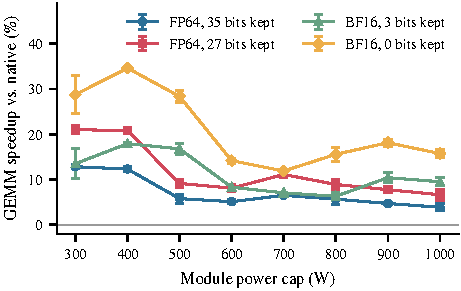
\includegraphics[width=\columnwidth]{figs/gemm_caps.pdf}
\caption{GEMM speedup from mantissa zeroing under module power caps (FP64 $32768{\times}32768{\times}2048$, BF16
$32768{\times}32768{\times}6144$; 95\pct{} paired intervals, 3 nodes $\times$ ABBA).}\label{fig:gemm}
\end{figure}

Zeroing speeds up GEMM at every cap, and more at lower caps (Fig.~\ref{fig:gemm}). FP64 keeping 27 bits is
$9.1\pm1.0$, $8.1\pm0.3$, $11.1\pm0.3$ and $8.9\pm1.0\pct$ faster at 500, 600, 700 and 800\W{} (95\pct{} intervals,
6 paired samples per point), an equivalent saving $\Delta W$ of 79--162\W; BF16 keeping 0 bits is 11.9--28.3\pct{}
faster, $\Delta W$ from 121\W{} to above 200\W. The most energy-efficient cap also shifts: native FP64 peaks at
500\W{} with 82\,GFLOP/J and the zeroed version reaches 107\,GFLOP/J; native BF16 peaks at 600\W{} with
950\,GFLOP/J, zeroed 1159\,GFLOP/J.

Against quantizing to FP8 (575\W, relative to native BF16), BF16 zeroed to 0 bits gives 1.15$\times$, native FP8
E4M3 1.87$\times$ and FP8 zeroed to 0 bits 2.12$\times$. FP8 E4M3's error of about 3.7\pct{} equals BF16 truncated
to 4 bits ($\approx$3.8\pct) or rounded to nearest at 3 bits ($\approx$3.5\pct). On narrow-range data, including
the real Llama\,2 70B weights, FP8 wins in both speed and accuracy. On data whose rows span $2^{-24}$ to $2^{24}$,
however, FP8 flushes 63\pct{} of the values to zero (median elementwise error 100\pct) while the Frobenius error is
only 3.9\pct; BF16 keeps every value's magnitude even at 0 bits.

\subsection{HPL and HPL-MxP on 8 Nodes}\label{sec:hpl}

\begin{table}[t]
\caption{HPL scaled residuals on 8 nodes (threshold 16; two runs per cell reproduce exactly).}\label{tab:hpl}
\centering\footnotesize\setlength{\tabcolsep}{4pt}
\begin{tabular}{@{}rrrrrr@{}}
\toprule
$N$ & Native & 36 bits & 28 bits & 24 bits & 20 bits \\
\midrule
131072 & $\ee{1.5}{-4}$ & 0.16 & 13.97 & 456 (F) & 9510 (F) \\
196608 & $\ee{1.3}{-4}$ & 0.073 & \textbf{18.09 (F)} & 463 (F) & 2850 (F) \\
262144 & $\ee{2.6}{-5}$ & 0.042 & 14.70 & 91 (F) & 599 (F) \\
\bottomrule
\end{tabular}
\end{table}

The HPL residual check determines the usable bit count, and it must be checked at several sizes
(Table~\ref{tab:hpl}). 28 bits sits on the failure edge and is not an operating point; 36 bits leaves a margin above
100$\times$. With 36 bits at $N=262144$, HPL is 3.4--8.3\pct{} faster at 400--800\W{} (Fig.~\ref{fig:hpl}),
$\Delta W=39$--97\W, and uses 4.3--7.7\pct{} less energy; at 1000\W{} it is only 0.7\pct{} faster but uses 7.7\pct{}
less energy per solve. (28 bits is 5.6--11.9\pct{} faster at the sizes where it passes; we list it only as a
boundary reference.)

\begin{figure}[t]
\centering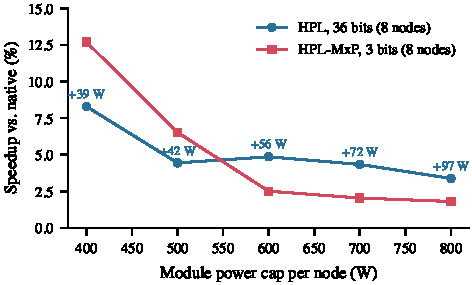
\includegraphics[width=\columnwidth]{figs/hpl_caps.pdf}
\caption{8-node HPL (36 kept bits, $N=262144$) and HPL-MxP (3 kept bits, $N=491520$) speedups; labels give the
equivalent power saving $\Delta W$ of HPL per node.}\label{fig:hpl}
\end{figure}

HPL-MxP (BF16 LU with FP64 refinement) has a similar boundary, and we use 3 kept bits. This is stable at all four
sizes $N=245760$--491520 (residual 1.4--3.8, always 3 refinement iterations). At $N=491520$ it is
12.7/6.5/2.5/2.0/1.8\pct{} faster at 400/500/600/700/800\W, $\Delta W=34$--45\W, with 3.4--10.7\pct{} less
energy; above 600\W{} the gain shrinks to about 2\pct{} because refinement grows from 1 iteration (native) to 3.
Keeping 0 bits gives 7.1--26.0\pct{} ($\Delta W$ 72--146\W) at $N=491520$, but at $N=245760$ refinement jumps from
1 to 52 iterations and performance falls by 70\pct: passing the residual check does not imply being faster. With
fans at full speed, native HPL-MxP at 1000\W{} trips the chassis hardware power brake (4--10\,s each time) while the
zeroed version, with lower peak power, never does; we exclude the 1000\W{} point from speedups.

\subsection{Plane-Wave DFT and Quantum Chemistry}\label{sec:sci}

Plane-wave DFT is tolerant. With 28 kept bits, the total energies of QE Si\,1000 and Au\,112 move by
$\ee{1.0}{-5}$ and $\ee{2.3}{-5}$\Ry{} under truncation and by $\ee{3.5}{-7}$ and $\ee{2.8}{-7}$\Ry{} under
round-to-nearest. The gold surface still converges at 20 bits with nearest rounding ($\ee{5.5}{-5}$\Ry, both runs);
for Si\,1000, 20 bits is the failure edge (one run converges with $\ee{1.1}{-4}$\Ry, the other aborts at iteration
24), and truncation diverges or slows at 20 bits. Gaussian-basis quantum chemistry needs more bits. GPU4PySCF
valinomycin DFT errs by $\ee{1.1}{-8}$\Eh{} at 44 bits; at 36 bits the energy oscillates near $10^{-8}$\Eh{} and
cannot meet a $10^{-10}$ convergence threshold, but with the chemically sufficient $10^{-7}$ threshold 40, 36 and 32
bits converge in the same 12 iterations as native, with a 32-bit nearest error of $\ee{1.2}{-5}$\Eh{}
($\approx$0.007\,kcal/mol). The error is then set by the threshold, not the bit count, consistent with the
$\approx$37 significant bits found sufficient by Dawson et al.~\cite{Dawson2024}.

Under caps, with the shim truncating every GEMM and compared against a baseline that takes the same copy path
without truncating, Si\,1000 at 550\W{} with 28-bit nearest rounding is 6.2\pct{} faster and uses 6.4\pct{} less
energy (SM clock 1348$\to$1446\,MHz), and Au\,112 at 450\W{} is 4.9\pct{} faster with 5.1\pct{} less energy.
These are upper bounds for a library that truncated internally; against the unmodified program the shim is
0.4\pct{} slower (Au\,112, 450\W) because of its $\approx$5\pct{} copy cost. The in-program version of
Section~\ref{sec:adaptive} truncates only Davidson blocks without copies and is the deployable number.

For GPU4PySCF, nsys shows FP64 GEMM kernels at 46\pct{} of GPU kernel time and 32\pct{} of total runtime for
valinomycin DFT (31\pct{} and 27\pct{} of kernel time for taxol and tamoxifen); the rest is dominated by copies of
computed intermediates (37--50\pct) and integrals. With 32--36 bits needed and FP64 GEMM keeping 35 bits
5.1--6.5\pct{} faster at 500--800\W, truncation alone is bounded at about $32\pct\times5$--$6.5\pct\approx1.6$--2.1\pct{}
end to end (3.9\pct{} at 400\W). This bound does not imply that truncation beats INT8 emulation here: the two
dominant GEMM shapes favor different methods (Section~\ref{sec:crossover}), and choosing by shape bounds the gain at
about 3.5\pct{} with cuBLAS emulation for the long-$k$ shape, or 6.6\pct{} with the less accurate GEMMul8.

\subsection{Tolerance-Driven Bit Counts in Quantum ESPRESSO}\label{sec:adaptive}

\begin{table}[t]
\caption{Quantum ESPRESSO with in-program truncation of Davidson blocks: mean $\pm$ 95\pct{} $t$ interval over 6
interleaved pairs ($m=2$: 2 runs). Energy integrates 1-s averaged module power.}\label{tab:qe}
\centering\footnotesize\setlength{\tabcolsep}{2.5pt}
\begin{tabular}{@{}llrrcc@{}}
\toprule
System & Setting & Time & Energy & $\Delta E$ (Ry) & SCF \\
\midrule
\multirow{4}{*}{\shortstack[l]{Au\,112\\(450\W)}} & Native & 92.4\,s & 35.8\,kJ & --- & 28 \\
 & Adapt.\ $m{=}0$ & $-4.2\pm0.7\pct$ & $-3.9\pm1.1\pct$ & $<10^{-8}$ & 28 \\
 & Adapt.\ $m{=}2$ & $-3.7\pct$ & $-2.9\pct$ & $<10^{-8}$ & 28 \\
 & Fixed 24 & $-2.7\pm1.1\pct$ & $-2.7\pm1.6\pct$ & $3{\times}10^{-8}$ & 28 \\
\midrule
\multirow{4}{*}{\shortstack[l]{Si\,1000\\(550\W)}} & Native & 211.1\,s & 111.8\,kJ & --- & 24 \\
 & Adapt.\ $m{=}0$ & $-2.4\pm0.5\pct$ & $-2.5\pm0.6\pct$ & $<10^{-8}$ & 24 \\
 & Adapt.\ $m{=}2$ & $-1.6\pct$ & $-1.6\pct$ & $<10^{-8}$ & 24 \\
 & Fixed 28 & $-2.3\pm0.6\pct$ & $-2.3\pm0.6\pct$ & $<10^{-8}$ & 24 \\
\bottomrule
\end{tabular}
\end{table}

The adaptive rule truncates the wavefunction blocks before and after applying the Hamiltonian in the Davidson
diagonalization. It reproduces the native total energy in every printed digit ($10^{-8}$\Ry) on both systems with
the same number of SCF iterations, while cutting time by 2.4--4.2\pct{} and module energy by 2.5--3.9\pct{}
(Table~\ref{tab:qe}); on the gold surface $k$ rises from 16 to 39 as the SCF converges. The results are unchanged for
three reasons. SCF is a self-correcting fixed-point iteration that already solves early iterations to a loose
$\mathit{ethr}$, and the rule keeps the truncation error ($\approx2^{-k}$) below the current threshold, so later
iterations correct it. In the last iterations $\mathit{ethr}\approx10^{-12}$ and $k\approx39$, and the total
energy is second order in the wavefunction error. And $10^{-8}$\Ry{} on a total of about $10^4$\Ry{} is a relative
$10^{-12}$. Fixed 24 bits is coarser than the threshold late in the SCF and leaves $\ee{3}{-8}$\Ry.

On the gold surface the adaptive rule beats fixed 24 bits in all 6 pairs by 0.6--1.8 points with no energy error,
because early iterations can use 16 bits. On Si\,1000 it beats fixed 28 bits in all 6 pairs, but only by
$0.18\pm0.14$ points. Its main value is that no safe bit count must be known in advance: one margin leaves both
systems unchanged and matches or beats the best fixed count, which can only be found after the fact. Unlike Woo et
al.\ and Huang et al., the arithmetic stays on native FP64 units with one-bit granularity, the signal is the
Davidson threshold, and the gain is clock headroom under a cap rather than a higher-throughput format.

\subsection{A Power-Bound Application: DF-MP2}\label{sec:mp2}

The codes above do not fill a 1000\W{} cap (Quantum ESPRESSO averages about 490--670\W). the density-fitted MP2 module of
GPU4PySCF~\cite{Wu2025} does: during MP2 the GPU draws about 800\W{} and the module 869--876\W, and matrix multiplication
takes 78\pct{} of GPU kernel time, nearly all of it the contraction $g_{ab}=B_iB_j^{\mathsf T}$ over slices of the
three-index tensor $B$ (FP64 DGEMM whose inner dimension is the auxiliary basis). We zero $B$ in place once after it
is built, so every later contraction benefits without copies, and compare with GPU4PySCF's built-in FP32 path and
cuBLAS emulation. One process runs DF-RHF once and then the variants interleaved (taxol def2-TZVP, 113 atoms, 2228
basis functions; two rounds per cap that differ by less than 0.6 points).

\begin{table}[t]
\caption{DF-MP2 (taxol def2-TZVP): speed relative to native in two rounds, and the error of the MP2 correlation
energy. At 1000\W{} the truncated variants run at native speed and draw 61--70\W{} (32 bits) and 106--115\W{}
(20 bits) less, using 7.7--8.6\pct{} and 13.7--14.4\pct{} less energy.}\label{tab:mp2}
\centering\footnotesize\setlength{\tabcolsep}{2.2pt}
\begin{tabular}{@{}lrllll@{}}
\toprule
Cap & Native & 32 bits & 20 bits & FP32 & Emu.\ 32 \\
\midrule
1000\W & 39.5\,s & $\pm0\pct$ & $\pm0\pct$ & +2.6/+11.5\pct & $-36\pct$ \\
700\W & 44.1\,s & +5.0/+5.5\pct & +7.4/+7.7\pct & +17.8/+18.3\pct & $-28\pct$ \\
500\W & 52.0\,s & +5.0/+4.7\pct & +8.6/+8.1\pct & +15.1/+14.9\pct & $-18\pct$ \\
\midrule
$|\Delta E|$ (E$_\mathrm{h}$) & --- & 1.2--$\ee{1.6}{-11}$ & $\ee{1.2}{-8}$ & 2.8--$\ee{4.2}{-8}$ & \\
\bottomrule
\end{tabular}
\end{table}

Keeping 32 bits changes the MP2 correlation energy by about $10^{-11}$\Eh{} and 20 bits by $\ee{1.2}{-8}$\Eh{}
(Table~\ref{tab:mp2}); the gains are on par with HPL. The built-in FP32 path is faster still, and its error of a few
$10^{-8}$\Eh{} is within chemical accuracy: the tensor's exponent span is narrow (27 binades overall, a median of
18 within a row), so FP32 fits (Section~\ref{sec:span}). cuBLAS emulation is 18--36\pct{} slower than native at this
shape ($m=n=2002$, $k=5477$).

\subsection{FP64 Beyond GEMM}\label{sec:nongemm}

Ozaki-type emulation applies only to dense matrix multiplication, so we also measured FP64 work that bypasses the
tensor cores (Table~\ref{tab:nongemm}). The benefit depends on how many operations separate the truncation point
from the multiplier and on what share of the data traffic is truncated. In the FMA loop the inputs feed the
multiplier directly; in N-body the position differences regrow full mantissas, and masking the intermediates inside
the loop costs more issue slots than it saves; a copy speeds up only when its bandwidth is power-capped; and in CG
the vectors dominate the traffic and the indices cannot be truncated. CG keeps the same 490 iterations, with a true
residual of $\ee{4}{-9}$ at 36 bits.

\begin{table}[t]
\caption{FP64 kernels without tensor cores: speedup at 400--700\W{} with 36 and 20 kept bits, and module power
saved at 1000\W{} with 20 bits.}\label{tab:nongemm}
\centering\footnotesize\setlength{\tabcolsep}{4pt}
\begin{tabular}{@{}lccr@{}}
\toprule
Kernel & 36 bits & 20 bits & Saved \\
\midrule
FMA loop & +2.7--4.8\pct & +5.6--9.0\pct & 138\W \\
N-body, inputs only & +1.3--2.0\pct & +2.6--3.9\pct & 59\W \\
N-body, also in loop & \multicolumn{2}{c}{$-6.5$ to $-11\pct$} & 60\W \\
Memory copy (450\W) & +7.7\pct & +14.0\pct & 70\W \\
CG, matrix values & \multicolumn{2}{c}{$\le$+1.7\pct} & 7\W \\
\bottomrule
\end{tabular}
\end{table}

\textbf{Third-party codes.} We zeroed, once at setup, the coefficient arrays that are stored and multiplied in every
step in three GPU FP64 codes: MFEM's partial-assembly quadrature data (about 43\pct{} of CG memory traffic), SW4's
material parameters (about 9\pct) and LAMMPS EAM tables (cache resident). Without zeroing all three are bitwise
identical to the originals or within rerun noise. MFEM (38.27\,M unknowns, $p=3$) is 0.9/2.0\pct{} faster with
36/20 bits (nearest) at 450\W{} and 0.7/1.4\pct{} at 550\W, unchanged at 1000\W; the solution changes by at most
$\ee{2.3}{-11}$. SW4 (126\,M grid points) is 0.6/1.3\pct{} faster at 350\W{} and 0.3/0.5\pct{} at 450\W{}, with
receiver waveforms changing by at most $\ee{3.4}{-11}$/$\ee{3.4}{-6}$ (doubling the grid changes them by 4--10\pct);
LAMMPS EAM (16.38\,M atoms) moves 0.0--0.4\pct, within noise. The gain order, MFEM $\ge$ SW4 $>$ LAMMPS, follows
the coefficients' share of memory traffic: kernel-level gains of 7--18\pct{} are diluted by the rest of the
full-mantissa computation. Zeroing fits best when inputs flow directly and in volume into multipliers or data
paths.

%==================================================================================================
\section{When Format Changes Win and When They Fail}\label{sec:format}

\subsection{Range versus Precision}\label{sec:range}

From the exponent histograms recorded by the shim (central 99.9\pct), operands span 12--14 binades in HPL, about 13
in Llama\,2 70B weights, 71--93 in Quantum ESPRESSO, 55--64 in GPU4PySCF taxol and 371--690 in valinomycin (down to
$2^{-691}$, beyond even FP32's range). Every scientific code fills the FP64 mantissa, so how many bits are needed
can only be found by zeroing experiments. Placing range against needed bits, plane-wave DFT (wide range, modest
precision) is the best target for mantissa zeroing, quantum chemistry needs both, and LLMs and HPL have narrow
ranges and can move to smaller formats.

\subsection{Crossover with INT8 Emulation of FP64}\label{sec:crossover}

cuBLAS~13 includes an Ozaki-type FP64 fixed-point emulation with a settable number of mantissa bits. On the same
node and cap we compare truncated native FP64 with emulation at similar error ($32768{\times}32768{\times}2048$,
400--1000\W, ABBA). Emulation works in slices of about 8 bits (24 and 28 bits give identical results,
$\ee{2.3}{-9}$). On this square-ish shape, three slices ($\ee{5}{-7}$) beat truncation to 20 bits by 51--73\pct; four
slices ($\ee{2}{-9}$) beat 28 bits by 6\pct{} at 1000\W{} to 23\pct{} at 400\W; at $10^{-11}$ truncation (about 36
bits) is 11--28\pct{} faster than five slices; and at $10^{-13}$ and below truncation is more than 40\pct{} faster.
The crossover is thus near 28--32 needed bits, and lower caps favor emulation---but only for this shape.

\begin{table}[t]
\caption{The two GEMM shapes that each carry 35\pct{} of valinomycin DFT flops: tall-skinny
$757248{\times}300{\times}2958$ and long-$k$ $2958{\times}2958{\times}76800$ (TFLOP/s; relative error in parentheses;
GEMMul8 errs by $\ee{1.0}{-10}$ and $\ee{8.2}{-10}$ on the two shapes).}\label{tab:shape}
\centering\footnotesize\setlength{\tabcolsep}{4pt}
\begin{tabular}{@{}lrrrr@{}}
\toprule
& \multicolumn{2}{c}{Tall-skinny} & \multicolumn{2}{c}{Long $k$} \\
\cmidrule(lr){2-3}\cmidrule(l){4-5}
Method & 1000\W & 575\W & 1000\W & 575\W \\
\midrule
FP64 native & 51.6 & 36.8 & 50.6 & 36.2 \\
Truncation, 36 bits ($\ee{1.0}{-11}$) & 54.0 & 38.9 & 53.7 & 38.0 \\
cuBLAS emu., 32 bits ($\ee{9.7}{-12}$) & 19.5 & 16.6 & 65.4 & 46.0 \\
cuBLAS emu., 28 bits ($\ee{2.3}{-9}$) & 24.2 & 20.9 & 89.9 & 65.6 \\
GEMMul8, 10 moduli & 17.9 & 16.7 & 102 & 75.6 \\
\bottomrule
\end{tabular}
\end{table}

\textbf{The crossover depends on shape.} Intercepting all 45,574 GEMMs of the valinomycin DFT run reveals two
shapes that each carry 35\pct{} of the flops (Table~\ref{tab:shape}). With $n=300$, emulation cannot amortize its
splitting and scaling: even at 28 bits it runs at less than half of native speed, and truncation wins at every
accuracy. With $k=76800$ the fixed costs amortize: emulation is still 21--22\pct{} faster than truncation at the
$10^{-11}$ level, and GEMMul8 (errors $\ee{1.0}{-10}$ and $\ee{8.2}{-10}$ on the two shapes) is nearly twice as fast at
$10^{-9}$. Within one application the best choice is per call: truncation for tall-skinny shapes, emulation for long
$k$.

\begin{figure*}[t]
\centering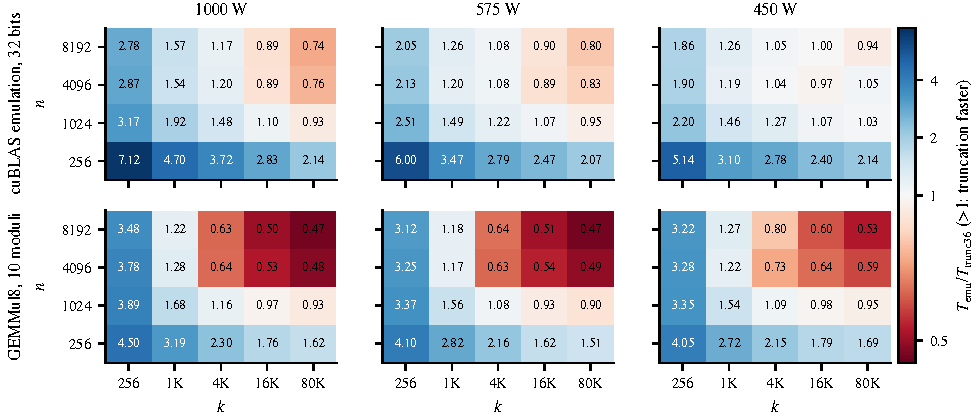
\includegraphics[width=\textwidth]{figs/crossover.pdf}
\caption{Time of INT8 emulation relative to truncation to 36 bits, $T_\mathrm{emu}/T_\mathrm{trunc36}$ ($m=8192$;
blue: truncation faster). Top: cuBLAS emulation with 32 bits; bottom: GEMMul8 with 10 moduli; columns: module
caps. Means of two rounds.}\label{fig:crossover}
\end{figure*}

\textbf{A shape sweep and a predictive model.} We fixed $m=8192$ and swept $n\in\{256,1024,4096,8192\}$ and
$k\in\{256,1024,4096,16384,81920\}$ at 1000, 575 and 450\W, two rounds each (480 records; Fig.~\ref{fig:crossover}).
Truncation to 36 bits beat native in all 60 shape--cap combinations (3.8--11.9\pct{} at 450\W, 3.6--5.9\pct{} at
575\W, 0.5--4.8\pct{} at 1000\W). cuBLAS emulation with 32 bits wins roughly when $n\ge4096$ and $k\ge16384$ (at
best 0.74$\times$ truncation time at 1000\W), and its winning region shrinks at lower caps: 5 of 20 shapes at 1000
and 575\W, 2 at 450\W. GEMMul8 with 10 moduli needs only 0.47--0.80$\times$ the truncation time when $n,k\ge4096$,
at an order of magnitude larger error ($\approx10^{-10}$ versus $10^{-11}$), and is up to 4.5$\times$ slower when $n$ or
$k$ is small. Emulation's extra work is input splitting ($\propto mk+nk$) and output accumulation ($\propto mn$);
dividing by the $mnk$ multiply gives
\begin{equation}
T_\mathrm{emu}/T_\mathrm{trunc} = A + B\,(1/m + 1/n) + C/k,
\end{equation}
where $A$ is the ratio of per-flop speeds. Least-squares fits per cap reach $R^2=0.98$--0.99 for GEMMul8, versus
0.86--0.89 for a single effective size $1/(1/m+1/n+1/k)$, so input and output costs must be separated; cuBLAS
emulation reaches 0.88--0.89, the residual likely reflecting different internal kernels per shape. On the two held-out
valinomycin shapes (two caps $\times$ two methods), the model picks the winner in 8 of 8 cases, with ratio errors of
7--16\pct{} for cuBLAS and 24--37\pct{} for GEMMul8 ($m=757248$ lies far outside the fitted range). On GH200 the choice
of emulation can thus be made in advance from $(m,n,k)$ and the cap, and truncation is a default that is never slower
than native.

\begin{table}[t]
\caption{Square GEMM ($32768{\times}32768{\times}2048$) in TFLOP/s by cap, ordered by relative error.}\label{tab:methods}
\centering\footnotesize\setlength{\tabcolsep}{4pt}
\begin{tabular}{@{}lrrr@{}}
\toprule
Method (error) & 1000\W & 575\W & 450\W \\
\midrule
Trunc., 36 bits ($\ee{1.0}{-11}$) & 61.8 & 45.5 & 38.6 \\
GEMMul8, 10 moduli ($\ee{1.0}{-10}$) & 70.8 & 51.4 & 34.7 \\
Trunc., 28 bits ($\ee{2.6}{-9}$) & 63.2 & 46.6 & 39.6 \\
GEMMul8, 9 moduli ($\ee{1.6}{-9}$) & 78.2 & 56.6 & 38.2 \\
cuBLAS emu., 28 bits ($\ee{2.3}{-9}$) & 67.8 & 55.2 & 47.5 \\
3xTF32 ($\ee{4.8}{-6}$) & 96.6 & 72.0 & 56.4 \\
FP32 SGEMM ($\ee{8.1}{-7}$) & 51.2 & 40.4 & 34.6 \\
\bottomrule
\end{tabular}
\end{table}

\textbf{The power of the emulation itself changes the winner.} GEMMul8 draws about 970\W{} at a 1000\W{} cap and at
450\W{} its clock drops to 650--720\,MHz, where truncation becomes faster; cuBLAS fixed-point emulation draws only
about 706\W{} at 1000\W{} and gains relative ground at lower caps (Table~\ref{tab:methods}). Truncation adds no work
and only lowers power, so it is most favorable under the tightest caps.

\subsection{FP32 and 3xTF32: Accumulation, Not Range}\label{sec:fp32}

3xTF32 is the fastest method in Table~\ref{tab:methods} but has only FP32-level accuracy, and its error grows with the
inner dimension: on $4096{\times}4096$ it is $\ee{6.4}{-7}$, $\ee{4.8}{-6}$ and $\ee{3.8}{-5}$ at $k=256$, 2048 and
16384, whereas FP32 SGEMM grows as $\sqrt{k}$ ($\ee{2.9}{-7}$, $\ee{8.1}{-7}$, $\ee{2.3}{-6}$) and FP64 truncation
is independent of $k$. The measured log slope of about one (7.5--7.9$\times$ per 8$\times$ in $k$) points to a
systematic error in TF32 tensor-core accumulation rather than random rounding, consistent with the round-toward-zero
accumulation Fasi et al.\ found on V100, T4 and A100~\cite{Fasi2021} (bit-accurate Hopper models:~\cite{Khattak2025}).
At $k=2048$ its error is more than ten times that of FP64 truncated to 20 bits ($\approx\ee{2.6}{-7}$).

Quantum ESPRESSO's operands fit in FP32's range, so we replaced every FP64 and complex FP64 GEMM with single
precision through the shim (inputs to FP32; 3xTF32 additionally splits into big and small parts multiplied three
times on TF32 tensor cores; $C$ combined in FP64). On the gold surface at 450\W{} (2 interleaved runs each), FP32
aborts at SCF iteration 26 and 3xTF32 and TF32 at iteration 2 when the Davidson bands fail to converge, and the
integrated charge drifts from 1232 electrons (FP32 $+0.012$, 3xTF32 $+0.074$); FP64 rounded to 24 and 20 bits
differs from native by $\ee{8.1}{-6}$ and $\ee{5.5}{-5}$\Ry{} and converges in 28 iterations. Si\,1000 at 550\W{}
behaves the same: FP32 aborts at iteration 14 and 3xTF32 at 9, with 4000.18 and 4001.52 electrons instead of 4000.
The difference is accumulation: truncated FP64 still accumulates in FP64, while Quantum ESPRESSO's inner dimension
is the number of plane waves (95386 on the gold surface plus a real GEMM with $k=4.3{\times}10^{6}$; 375286 for
Si\,1000), where 3xTF32 already errs by $\ee{5.6}{-5}$ to $\ee{2.2}{-4}$, the same order as plain TF32. FP32 GEMM on
Hopper is also slower than FP64 tensor cores (about 1.5$\times$ per SCF iteration). For long-inner-product solvers,
single precision is not an option even when the range fits; FP64 truncation is the reduced-precision choice that
leaves the algorithm unchanged.

\subsection{Exponent Span Decides Whether Formats Can Change}\label{sec:span}

Truncation keeps every element's 11-bit exponent and changes only its mantissa; format changes must handle the
exponent. Per-tensor scaled formats (FP32, FP8) need the whole tensor inside the format's range, and Ozaki-type INT8
emulation slices each row (column) relative to its maximum, so with $k$ kept bits elements more than $2^{-k}$ below
the row maximum are lost. The exponent span of the data therefore decides whether a format change is possible,
whereas truncation is unaffected.

\begin{figure}[t]
\centering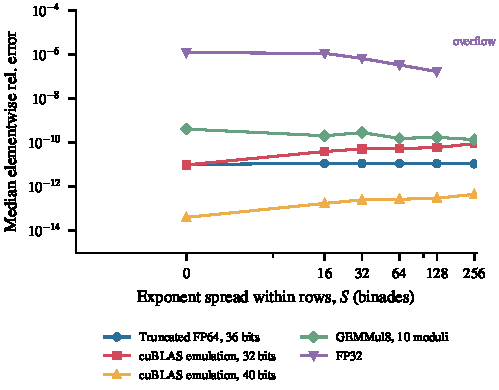
\includegraphics[width=\columnwidth]{figs/spread_error.pdf}
\caption{Synthetic exponent spread: elements of $8192{\times}8192{\times}16384$ operands have exponents uniform over
$S$ binades within each row (1000\W).}\label{fig:spread}
\end{figure}

\textbf{Synthetic data.} On $8192{\times}8192{\times}16384$, a shape where emulation is faster at narrow spans, we
draw element exponents uniformly over $S$ binades (1000/575\W, two rounds; Fig.~\ref{fig:spread}). Truncation to 36
bits keeps a median elementwise error of 1.0--1.1$\times10^{-11}$ and a speedup of 4.4--6.3\pct. cuBLAS emulation with
a fixed 32 bits degrades by 4--9$\times$ in median (7--19$\times$ at p99) and needs 2--3 more bits; its dynamic mode,
which targets FP64-equivalent accuracy, raises the bit count from 58 to 301 and effectively falls back to native at
1.6--2.2$\times$ the truncation time; FP32 overflows at $S=256$. GEMMul8 is barely affected on uniformly spread data.
If the spread is only between rows (one scale per row), emulation is unaffected while FP32 still overflows.

\begin{table}[t]
\caption{Real data (1000\W, one run each): flop-weighted fraction of nonzeros more than $2^{-32}$ below their row
maximum, and the total-energy error of each method.}\label{tab:span}
\centering\footnotesize\setlength{\tabcolsep}{4pt}
\begin{tabular}{@{}llll@{}}
\toprule
& Valinomycin & QE Si\,1000 & QE Au\,112 \\
\midrule
Below $2^{-32}$ & 24--44\pct & 0.24--0.54\pct & 0.008--0.02\pct \\
Trunc., 36 bits & $\ee{9.6}{-7}$\Eh & 0\Ry & 0\Ry \\
Trunc., 32 bits & $\ee{1.2}{-5}$\Eh & 0\Ry & $\ee{4}{-8}$\Ry \\
cuBLAS emu., 36/32 & $\mathbf{\ee{5.25}{-2}}$\,\textbf{E}$_\mathbf{h}$ & $\ee{6}{-8}$\Ry & $\ee{5}{-8}$\Ry \\
GEMMul8, 10 moduli & diverges & out of memory & $\ee{3.7}{-7}$\Ry \\
\bottomrule
\end{tabular}
\end{table}

\textbf{Real data.} The shim samples 256 rows of op($A$) and 256 columns of op($B$) per GEMM and records the fraction
of nonzeros more than $2^{-32}$ below their row maximum, weighted by flops (validated against theory on synthetic
data). In Gaussian-basis DFT the atomic-orbital values on the grid decay exponentially with distance, and in the worst
shape 87\pct{} of elements are more than $2^{-32}$ below their row maximum. There, 36-bit cuBLAS emulation lets the SCF
converge normally in 12 iterations to a total energy that is off by 52\,mE$_\mathrm{h}$ ($\approx$33\,kcal/mol), and
GEMMul8 diverges; truncation to the same 36 bits errs by $\ee{9.6}{-7}$\Eh{} (Table~\ref{tab:span}). On Quantum
ESPRESSO, with narrow per-row spans, the same emulation errs by only 5--$\ee{6}{-8}$\Ry. Uniform synthetic spreads
understate the problem; whether emulation is safe can be decided beforehand by measuring per-row spans
(Fig.~\ref{fig:map}). DF-MP2 (Section~\ref{sec:mp2}) sits at the other end: narrow span, and FP32 works.

\begin{figure}[t]
\centering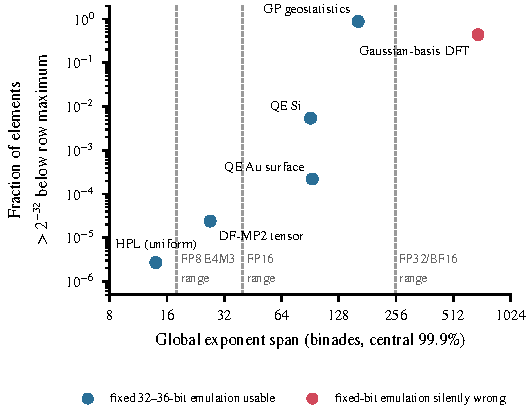
\includegraphics[width=\columnwidth]{figs/range_map.pdf}
\caption{Global exponent span against the fraction of elements more than $2^{-32}$ below their row maximum, with the
measured outcome of 32--36-bit cuBLAS emulation.}\label{fig:map}
\end{figure}

\textbf{Wide range, partly power-bound DFT.} These DFT runs draw only 650--690\W{} at 1000\W, but are power-bound
below that. For valinomycin (grid level 6) at 550 and 450\W, truncation to 36 bits through the shim is 3.3--3.5\pct{}
faster than the copy baseline with 2--3\pct{} less energy and an error of $\ee{9.5}{-7}$\Eh; emulation must keep 40 bits
to stay correct and then takes 1.48--1.53$\times$ the baseline time (two rounds each).

\subsection{Wide Range and Power-Bound: Gaussian-Process Geostatistics}\label{sec:gp}

Maximum-likelihood estimation of a Gaussian process in geostatistics factors an $n{\times}n$ Matérn covariance matrix
by Cholesky at every likelihood evaluation. As in HPL, almost all work is FP64 matrix multiplication, but the
covariance decays exponentially with distance. We implemented an ExaGeoStat-like kernel: $n=80000$ random 2-D
locations, Matérn-3/2 covariance (nugget $10^{-4}$), blocked Cholesky ($n_b=1024$, trailing updates by cuBLAS DGEMM),
and the log-likelihood at six range parameters (0.02--0.08). Each panel $L_{21}$ keeps $k$ bits in place before the
trailing update; we compare with cuBLAS emulation and FP32 (1000/700/500\W, two interleaved rounds). Native draws
947--955\W{} of module power at 1000\W{} and is capped 86--91\pct{} of the time, and 88\pct{} of the panels' nonzeros
are more than $2^{-32}$ below their row maximum.

\begin{table}[t]
\caption{Gaussian-process likelihood ($n=80000$, six range parameters): largest log-likelihood deviation from
native and speed relative to native (two rounds). At 1000\W{} truncation runs at native speed and uses
3.6--4.0\pct{} (36 bits) and 8.8--9.9\pct{} (28 bits) less energy.}\label{tab:gp}
\centering\footnotesize\setlength{\tabcolsep}{3pt}
\begin{tabular}{@{}lllll@{}}
\toprule
 & Trunc.\ 36 & Trunc.\ 28 & cuBLAS emu.\ 36 & FP32 \\
\midrule
$\max|\Delta\ell|$ & $\ee{2.4}{-5}$ & $\ee{7.2}{-4}$ & $\ee{2.2}{-3}$ & 87 \\
1000\W & $\pm0\pct$ & $\pm0\pct$ & $-40\pct$ & $-9\pct$ \\
700\W & +2.7/+3.2\pct & +5.5/+5.7\pct & $-32\pct$ & +2.3\pct \\
500\W & +2.8/+3.3\pct & +5.2/+5.7\pct & $-22\pct$ & +4.7\pct \\
\bottomrule
\end{tabular}
\end{table}

The log-likelihood is about 1.2--1.7$\times10^5$, so a deviation of $\ee{7.2}{-4}$ at 28 bits is far below what
matters for estimation (Table~\ref{tab:gp}); the 1000\W{} figures use the second round, because the first native run
includes warm-up. FP32's deviation stems mainly from the conditioning of the covariance at long ranges and makes it
unusable for estimation. cuBLAS emulation is slower than truncation at this shape ($k=1024$) and less accurate than
28-bit truncation. The per-row span is wider than in the DFT case, yet emulation does not go wrong, only loses
accuracy: a wide per-row span is necessary but not sufficient for emulation failure, which also depends on how much
the dropped small elements contribute.

\textbf{A complete maximum-likelihood fit.} To check that the estimate itself is unchanged, we ran the whole fit:
golden-section search over the log range parameter, 17 likelihood evaluations per variant ($n=60000$; 1000 and
700\W; two interleaved rounds). Truncation to 36 and 28 bits and cuBLAS emulation return the native estimate
$\hat\theta=0.05007952$ in every printed digit, with maximized log-likelihoods within $\ee{4.8}{-6}$ (36 bits) and
$\ee{2.3}{-4}$ (28 bits) of native; FP32 moves $\hat\theta$ by 0.49\pct{} and loses 0.72 in log-likelihood (at
$n=8000$ even FP32 agrees, so its error grows with the problem). At 700\W{} the fit is 5.2\pct{} faster with 28 bits
and 2.5\pct{} faster with 36 bits in both rounds, using 5.0\pct{} and 2.7\pct{} less energy; at 1000\W{} it runs at
native speed with 6.7--7.1\pct{} and 1.6--3.0\pct{} less energy; cuBLAS emulation is 31--41\pct{} slower. Among
whole-matrix choices, truncation is the only one that is both fast and accurate on this wide-range, power-bound workload.

\textbf{Composing with tile mixed precision.} The mixed-precision Cholesky factorizations of the ExaGeoStat line change
the format of whole tiles instead (Section~\ref{sec:related}). To see whether truncation still helps there, we ordered
the locations along a Morton curve and added such a variant to our kernel: in the trailing update, tiles below each
column's FP64 extent, chosen by the tile-norm rule with a required accuracy of $10^{-9}$ as in~\cite{Cao2023}, use FP16
inputs with FP32 accumulation on the tensor cores (52\pct{} of the tiles at range 0.02, 3\pct{} at 0.08). Over the six
ranges ($n=60000$, two ABBA rounds) it runs 1.60--1.63$\times$ faster than native FP64 at 1000, 700 and 500\W, with
log-likelihood deviations up to 0.043. Truncating its remaining FP64 tiles to 28 bits makes it another 1.9\pct{}
faster at 1000\W{} and 6.2--7.1\pct{} faster at 700 and 500\W, with an unchanged deviation, so truncation composes with
format changes rather than competing with them. Zeroing the FP16 operands to 5 mantissa bits as well added nothing.

\textbf{ExaGeoStat itself.} We also built ExaGeoStatCPP (StarPU and Chameleon tile Cholesky with cuBLAS; tile size
1920) and ran its MLE ($N=60000$, six BOBYQA evaluations per run, data generated once natively and read by every run)
with the shim on its FP64 tile GEMMs. Matérn covariance generation runs on the CPU and takes about 9\,s per evaluation
against 2.3\,s of GPU factorization at 1000\W, and the factorization is partly power-limited even there (GPU power
650--690\W, frequent power-cap events). Relative to a baseline that copies the operands without truncating, truncation
shortens the factorization by 3.0\pct{} (36 bits) and 4.0\pct{} (28 bits) at 1000\W, 5.0\pct{} and 8.0\pct{} at
600\W, and 5.6\pct{} and 9.4\pct{} at 450\W{} (two ABBA rounds); with 28 bits the mean SM clock during
factorization rises from 1913 to 1975\,MHz at 1000\W{} and from 1166 to 1305\,MHz at 600\W. The
log-likelihoods change by at most $\ee{1.2}{-10}$ and $\ee{9.8}{-8}$ relative. The shim's own copy costs 7--9\pct, which
leaves it at parity with unmodified ExaGeoStat (28 bits: $-3.1$, $-1.3$ and $-0.5\pct$), so the gain needs an
implementation inside the library.

%==================================================================================================
\section{AI Workloads: Training and Inference}\label{sec:ai}

MLPerf Training measures time to target quality (eval loss $\le0.925$ on GovReport for Llama\,2 70B LoRA); a faster
step that needs more samples to converge loses.

\textbf{Training: truncating the FP8 base weights is a negative result.} We truncated only the frozen FP8 base weights
of Llama\,2 70B LoRA (once, after loading); activations, gradients, LoRA weights and updates and per-tensor scaling
follow~\cite{Micikevicius2022}. On 8 nodes with the same seed, native FP8 at 575\W{} reached the target after 3456
samples in 28.34\,min. Keeping 2 bits made each 384 samples only 0.9--1.2\pct{} faster but needed 4224 samples (22\pct{}
slower at 575\W, 19\pct{} at 800\W); 1 bit did not converge. The train-loss gap appears at the first logged step and
stays constant, and the eval-loss curve shifts up by 0.007--0.008: truncation weakens the base model at load time,
and a rank-16 adapter does not compensate. A second seed (5678, 800\W) agrees: native 3072 samples in 22.74\,min,
2 bits 4224 samples in 31.56\,min (+39\pct). Across two seeds and three pairs, the first evaluation is always
0.008--0.010 higher and convergence takes 2--3 more evaluation intervals. Native convergence differs by one interval
between node sets (3072 versus 3456), so we read this only as evidence that FP8's 3 mantissa bits leave no room. The
rounding mode shows no consistent order (at 800\W{} truncation and stochastic rounding converge at 4224 samples,
nearest at 5376). Truncating only MLP layers needs 4224 samples, attention only 3840 (one interval, within node-set
noise, but attention is only about 18\pct{} of the linear weights); the first-evaluation gaps of $+0.0064$ (MLP) and
$+0.0028$ (attention) add up to the $+0.0086$ of full truncation. A repeat of the attention-only run gave nearly the
same first evaluation (0.9428 versus 0.9425) but converged one interval later (4224 versus 3840, missing the target by
$10^{-5}$ at 3840), so the first-evaluation gap, not the convergence point, is the robust metric.

\begin{table}[t]
\caption{WikiText-2 perplexity (sequence 2048) relative to BF16 for the linear layers' formats; FP8 uses real FP8
tensor-core GEMMs.}\label{tab:llm}
\centering\footnotesize\setlength{\tabcolsep}{2.2pt}
\begin{tabular}{@{}lrrrrrr@{}}
\toprule
Format & L2-7B & L3.1-8B & Qw2.5-7B & Mis-7B & OPT-6.7B & L2-70B \\
\midrule
BF16, 4 b & +0.09 & +0.19 & +0.13 & +0.09 & +0.45 & +0.10 \\
BF16, 3 b & +0.44 & +1.02 & +0.65 & +0.41 & +2.00 & +0.51 \\
FP8 per tensor & +0.63 & +0.95 & +0.70 & +0.45 & +2.23 & +0.48 \\
FP8 per channel & +0.32 & +0.88 & +0.61 & +0.34 & +0.69 & +0.42 \\
FP8 p.c., 2 b & +3.2 & +6.5 & +4.0 & +2.5 & +7.0 & +3.4 \\
FP8, wts.\ 2 b & +1.9 & +4.0 & +2.6 & +1.3 & +2.8 & --- \\
\bottomrule
\end{tabular}
\\[2pt]{\scriptsize Values in percent. b: kept bits; L: Llama, Qw: Qwen, Mis: Mistral; p.c.: per channel; wts.: weights only.}
\end{table}

\textbf{Inference: FP8 has already taken most of the benefit.} BF16 rounded to nearest at 3 bits has as many mantissa
bits as FP8 E4M3 and matches its accuracy on six language models (Table~\ref{tab:llm}; with truncation, 4 bits are
needed). We then compared the two where FP8 is known to fail: attention perplexity at 2k/8k context (BF16 3 bits
$+0.49/+1.06\pct$, emulated FP8 attention $+0.52/+1.08\pct$), key retrieval at 8k--32k context on Llama-3.1-8B (both
100\pct), BERT-large SQuAD (all formats above 99.9\pct{} of FP32 F1) and CogVideoX-2B video generation (PSNR against
native 18--38\,dB for FP8 attention, 20--29\,dB for BF16 3 bits). With proper scaling the two tie, and FP8 is about
twice as fast. A naive FP8 attention that does not scale the softmax probabilities fails as sequences grow (74\pct{}
error at 4096 tokens), and on CogVideoX-2B (about 18k tokens) it changes the composition and adds noise (PSNR
10--12\,dB, SSIM 0.07--0.66) where BF16 with 3 bits keeps 20--21\,dB and SSIM 0.82--0.91. This is a range problem,
not a mantissa problem: the smallest positive E4M3 value, about $2^{-9}$, exceeds the mean attention probability over
18k tokens, while BF16 has 8 exponent bits; correct implementations already fix it inside FP8~\cite{Zhang2025}.

Zeroing on top of FP8 is the only way to go faster than FP8 on Hopper, which lacks FP4. On real layer-40 activations
and weights of Llama2-70B ($8192{\times}57344{\times}8192$), keeping 2 bits on both sides is 4.4/3.2/5.0/8.2\pct{}
faster at 1000/700/575/450\W, weights only 1.3--3.3\pct, but 70B perplexity rises by 3.4\pct. Per-layer sensitivity
shows q/k/v as least sensitive but only 7.8\pct{} of the compute each, and MLP layers as most of the compute but more
sensitive; every selection trades speed for accuracy at about the same rate. FP8's advantage comes mainly from halving
the data path: at 575\W{} BF16 with 3 bits is only 8\pct{} faster than BF16, while FP8 is 1.8$\times$. Power savings
are limited too. Decode (64 tokens) is bandwidth-bound and unchanged in speed at 1000\W; FP8 zeroed to 0 bits saves
104\W{} on uniform data but only 61\W{} on real Llama2-70B weights, and truncating weights to 2 or 0 bits saves only
1.5\pct{} or 5.5\pct{} of power at an accuracy cost. Below 575\W{} these savings turn into 2--16\pct{} speedups, and
prefill is power-bound even at 1000\W.

For weights and activations that directly set model quality and have no residual correction, zeroing turns directly
into quality loss, in contrast with solvers such as HPL-MxP and SCF that correct errors. For GPUs without FP8 tensor
cores, or pipelines that must stay in BF16, BF16 with 3--4 kept bits is a nearly lossless option; for FP8 deployments,
zeroing saves only 1.5--5.5\pct{} of power in memory-bound phases, at an accuracy cost.

%==================================================================================================
\section{Discussion}\label{sec:discussion}

\textbf{Benefit under a fixed power budget.} Under a power budget such as a student cluster competition's,
the equivalent power saving becomes usable compute. At 8 nodes $\times$ 700\W, HPL with the safe 36 bits rises from
331.6 to 346.0\,TFLOP/s (+4.3\pct); native HPL would need about 772\W{} per node, about 0.6\,kW more for the cluster,
to match. Without a cap the gain becomes energy at equal speed: 7.7\pct{} per HPL solve. The cost is one bit mask and
no hardware. At 575\W{} the SM clocks of our 14 nodes differ by 17\pct{} (1129--1325\,MHz), and synchronous runs move
at the pace of the slowest node; zeroing and per-node caps are complementary.

\textbf{Benchmark rules.} TOP500 HPL and HPL-MxP rules do not accept results computed on altered operand values, so
all HPL and HPL-MxP numbers here are research results, not official scores. MLPerf Inference closed division allows
any mathematical quantization but forbids pruning~\cite{MLPerfInfRules}; zeroing is the former. Whether MLPerf
Training permits truncated weights depends on each round's rules; in our results uniform truncation does not pay
anyway. Scientific software has no such restriction; the criterion is whether physical results stay within the
required accuracy.

\textbf{A hardware counterexample.} An Altera patent states that zeroing low bits at the input of an FPGA
floating-point multiplier ``barely reduces power'' because the compression tree keeps
switching~\cite{Altera2017}. This does not contradict our measurements: the patent is a qualitative statement about a
$27{\times}27$ fixed-point multiplier, whereas on a GPU the truncated bits also travel through registers, operand
buses and memory, whose toggles disappear as well. Table~\ref{tab:fill} supports this: a pure memory copy saves
18\pct{} of module power without any multiplication, 97\pct{} of it from the absence of toggles, while in the
multipliers zeros still save more than ones, so the GH200 multipliers also switch less when partial products are
constantly zero.

\textbf{Limitations and threats to validity.} (i)~All experiments use one GH200 cluster; other GPU generations are
not covered (an earlier report has preliminary H200 and MI350X results). (ii)~The HPL residual is a deterministic but
chaotic function of $N$: 28 bits passes at $N=131072$ and 262144 and fails at 196608, so our operating point is 36 bits
validated at several sizes; likewise 3 bits for HPL-MxP. (iii)~Each scientific code was tested on one input system;
forces, geometry optimization and larger systems are not covered. (iv)~The shim costs 3--6\pct{} for copies, so
shim results are always compared with a baseline taking the same copy path; in-program zeroing has no such cost.
(v)~Nodes differ by 13--17\pct{} at equal power, so all comparisons are paired on the same nodes by ABBA order or by
seed. (vi)~Cooling and the chassis supply change conclusions: at low fan speed the GPU hits its thermal limit first,
and at full fan speed native HPL-MxP at 1000\W{} trips the hardware power brake; these conditions must be reported.
(vii)~The cluster is shared and another user's tool once reset all caps, so every window checks the cap in effect.
(viii)~Power comes from the driver's sensor, not an external meter, and on A100/H100 it samples only part of the
time~\cite{Yang2024}; our comparisons are paired relative values on one measurement path with steady windows of
10--20\,s, but absolute energy should be cross-checked with an external meter. (ix)~The truncation-versus-emulation
comparisons of Section~\ref{sec:span} ran once per setting, and GEMMul8 ran out of GPU memory on two applications.
(x)~The Gaussian-process results come from our ExaGeoStat-like kernel on synthetic data, and its mixed-precision
variant is a simplified re-implementation (FP64 storage, one FP16 GEMM per panel over the tiles that need it), not the
ExaGeoStat code; ExaGeoStat itself was measured only through the shim, whose copy cost offsets the gain.

%==================================================================================================
\section{Conclusion}\label{sec:conclusion}

On a production GH200 cluster, truncating unused mantissa bits in software buys real performance for real HPC
applications under power caps without changing their physical results. On complete programs with correctness checks
at 400--800\W, HPL keeping 36 bits is 3.4--8.3\pct{} faster (39--97\W{} equivalent), HPL-MxP keeping 3 bits
1.8--12.7\pct, Quantum ESPRESSO with tolerance-driven bit counts 2.4--4.2\pct{} with bitwise-identical energies,
power-bound DF-MP2 4.9--8.3\pct, and wide-range, power-bound Gaussian-process geostatistics 5.2--5.7\pct; without a
cap HPL uses 7.7\pct{} less energy per solve. Microbenchmarks give upper bounds (FP64 GEMM keeping 27 bits:
6.6--21\pct; pure data movement: 18\pct{} less module power at 1000\W), not application operating points. The gain
comes mainly from fewer toggles in arithmetic units and data paths, so it suits FP64 solvers with residual correction
or self-consistent iteration whose inputs flow directly and in volume into multipliers. Its scope is also clear: the
crossover with INT8 emulation of FP64 moves with matrix shape and cap and can be predicted from $(m,n,k)$ by a
three-parameter model; data with a wide exponent span can only be truncated, since row-sliced emulation can silently
go wrong; FP32 and 3xTF32 are no substitute on long inner products; kernels whose intermediates regrow full mantissas
gain little; and for FP8 AI inference, further zeroing trades accuracy for speed. Mantissa zeroing adds no work, needs
no hardware support, and complements format changes. All numbers are research results, not official TOP500 or
MLPerf scores.

\bibliographystyle{IEEEtran}
\bibliography{refs}

\end{document}
